%%%%%%%%%%%%%%%%%%%%%%%%%%%%%%%%%%%%%%%%%
%%% HYPERRIDE Reporting Template
%%%%%%%%%%%%%%%%%%%%%%%%%%%%%%%%%%%%%%%%%

\documentclass[letterpaper,12pt]{report}
\usepackage[pass]{geometry}
\usepackage{istgame}
\usepackage{xcolor}
\usepackage{xurl}
\usepackage{hyperride}		% HYPERRIDE specific definitions and styles  
\usepackage[utf8]{inputenc}	% UTF8 package
\usepackage[T1]{fontenc}
\usepackage{textcomp}		% common special chars
\usepackage{amsmath}		% math formula
\usepackage{fancybox}
\usepackage{anyfontsize}	% fonts
\usepackage{lipsum}
\usepackage{float}
\usepackage[normalem]{ulem}
\usepackage{cleveref}
\usepackage[printonlyused]{acronym}
\hypersetup{
	pdftitle={Beacon Labs - Workshop},
	pdfauthor={[Dylan Gresham, Gaby Dagher, Jordan Whyte, Gunnar Vittrup, Josh Boyle]},
	pdfkeywords={Beacon Labs, Workshop, Cybersecurity, Middlebox, TCP Amplification, Network Security, Mobile Security, Web Security, Service Workers, XSS, Cross-Site Scripting, Android Vulnerability},
}
\usepackage{booktabs}
\usepackage{subfigure}
\usepackage{graphicx}
\usepackage{xcolor}
\usepackage{soul}
\sethlcolor{lightgray}
\usepackage[export]{adjustbox}
\usepackage{mdframed}
\usepackage{pdfpages}
\usepackage{comment}
\usepackage{multirow,array}
\def\todo#1{{\color{hyperridered}\textbf{TODO:} ``#1''}}
\def\hyperride{HYPERRIDE}
\definecolor{lightblue}{rgb}{0.87, 0.94, 1}
\graphicspath{ {graphics/} }

%%%%%%%%%%%%%%%%%%%%%%%%%%%%%%%%%%%%%%%%%
%%% Definitions
%%%%%%%%%%%%%%%%%%%%%%%%%%%%%%%%%%%%%%%%%

%% stuff for displaying code

% Define the listing package
\usepackage{listings} % code highlighter
\usepackage{color} % use color
\definecolor{mygreen}{rgb}{0,0.6,0}
\definecolor{mygray}{rgb}{0.5,0.5,0.5}
\definecolor{mymauve}{rgb}{0.58,0,0.82}

% Customize a bit the look
\lstset{ %
  backgroundcolor=\color{white}, % choose the background color; you must add \usepackage{color} or \usepackage{xcolor}
  basicstyle=\footnotesize, % the size of the fonts that are used for the code
  breakatwhitespace=false, % sets if automatic breaks should only happen at whitespace
  breaklines=true, % sets automatic line breaking
  captionpos=b, % sets the caption-position to bottom
  commentstyle=\color{mygreen}, % comment style
  deletekeywords={...}, % if you want to delete keywords from the given language
  escapeinside={\%*}{*)}, % if you want to add LaTeX within your code
  extendedchars=true, % lets you use non-ASCII characters; for 8-bits encodings only, does not work with UTF-8
  frame=tblr, % adds a frame around the code with line numbers inside the box
  keepspaces=true, % keeps spaces in text, useful for keeping indentation of code (possibly needs columns=flexible)
  keywordstyle=\color{blue}, % keyword style
  % language=Octave, % the language of the code
  morekeywords={*,...}, % if you want to add more keywords to the set
  numbers=left, % where to put the line-numbers; possible values are (none, left, right)
  numbersep=5pt, % how far the line-numbers are from the code
  numberstyle=\tiny\color{mygray}, % the style that is used for the line-numbers
  rulecolor=\color{black}, % if not set, the frame-color may be changed on line-breaks within not-black text (e.g. comments (green here))
  showspaces=false, % show spaces everywhere adding particular underscores; it overrides 'showstringspaces'
  showstringspaces=false, % underline spaces within strings only
  showtabs=false, % show tabs within strings adding particular underscores
  stepnumber=1, % the step between two line-numbers. If it's 1, each line will be numbered
  stringstyle=\color{mymauve}, % string literal style
  tabsize=2, % sets default tabsize to 2 spaces
  title=\lstname % show the filename of files included with \lstinputlisting; also try caption instead of title
}
% END of listing package %

\definecolor{darkgray}{rgb}{.4,.4,.4}
\definecolor{purple}{rgb}{0.65, 0.12, 0.82}

% Define Javascript language
\lstdefinelanguage{JavaScript}{
  keywords={typeof, new, true, false, catch, function, return, null, catch, switch, var, if, in, while, do, else, case, break},
  keywordstyle=\color{blue}\bfseries,
  ndkeywords={class, export, boolean, throw, implements, import, this},
  ndkeywordstyle=\color{darkgray}\bfseries,
  identifierstyle=\color{black},
  sensitive=false,
  comment=[l]{//},
  morecomment=[s]{/*}{*/},
  commentstyle=\color{purple}\ttfamily,
  stringstyle=\color{red}\ttfamily,
  morestring=[b]',
  morestring=[b]"
}

\lstset{
  language=JavaScript,
  extendedchars=true,
  basicstyle=\footnotesize\ttfamily,
  showstringspaces=false,
  showspaces=false,
  numbers=left,
  numberstyle=\footnotesize,
  numbersep=9pt,
  tabsize=2,
  breaklines=true,
  showtabs=false,
  captionpos=b
}

%%%%%%%%%%%%%%%%%%%%%%%%%%%%%%%%%%%%%%%%%
%%% Definitions
%%%%%%%%%%%%%%%%%%%%%%%%%%%%%%%%%%%%%%%%%
\newcounter{taskset}
\setcounter{taskset}{1} % Set the initial value of the taskset counter

\newcounter{action}[taskset]
\renewcommand{\theaction}{\thesection.\arabic{taskset}.\arabic{action}}

\newcommand{\myaction}[1]{%
  \refstepcounter{action}%
  \textbf{Action \theaction: #1}%
}


% CHANGE %'s below to make subsection headings visible/invisible in TOC
%\newcommand{\xsubsubsection}[1]{\subsection{#1}}
%\newcommand{\xsubsubsection}[1]{\subsubsection{#1}}

\setcounter{secnumdepth}{4}
\setcounter{tocdepth}{5}

\begin{document}


\includepdf[pages=1]{./graphics/2FP.pdf}

\mdfdefinestyle{code}{%
    linecolor=black,
    outerlinewidth=2pt,
    %roundcorner=20pt,
    innertopmargin=4pt,
    innerbottommargin=4pt,
    innerrightmargin=4pt,
    innerleftmargin=4pt,
    leftmargin = 4pt,
    rightmargin = 4pt
    backgroundcolor=black!10
}

\setcounter{tocdepth}{4}
\setcounter{secnumdepth}{4}

%%%%%%%%%%%%%%%%%%%%%%%%%%%%%%%%%%%%%%%%%
%%% URL style same as regular text
%%%%%%%%%%%%%%%%%%%%%%%%%%%%%%%%%%%%%%%%%
	
\urlstyle{same}

%%%%%%%%%%%%%%%%%%%%%%%%%%%%%%%%%%%%%%%%%
%%% Deliverable Information
%%%%%%%%%%%%%%%%%%%%%%%%%%%%%%%%%%%%%%%%%

% Project Meta Information
\ProjectFullTitle{Beacon Network Security Labs: Middlebox Amplification Attack Activity}
\ProjectAcronym{HYPERRIDE}
\ProjectRefNo{957788}

% Report Number, use either "1", "2", or "3" for the corresponding reporting period
\delivNumber{0}

% Period covered by the report
\delivFrom{dd/mm/yyyy}
\delivTo{dd/mm/yyyy}

% Report Responsible Partner
\delivResponsible{AIT Austrian Institute of Technology (AIT)} 

% Report Version, Contractual and Actual Date, Dissemination Level, Type
\delivVersion{vn.n}
\ContractualDate{dd/mm/yyyy}
\ActualDate{dd/mm/yyyy}

% List of Main Authors (usually from the responsible partner)
\delivAuthor{[Jordan Whyte, Gaby Dagher]}

% List of Co-Authors (all other co-authors should be listed here)
\delivFPAuthor{[]}

% Report Status
\delivStatus{d} %% d = draft, f = final, s = submitted

%%%%%%%%%%%%%%%%%%%%%%%%%%%%%%%%%%%%%%%%%
%%% Change Log
%%%%%%%%%%%%%%%%%%%%%%%%%%%%%%%%%%%%%%%%%

\istChange{dd/mm/yyyy}{v1.0}{Name (Partner short name)}{Draft report template}
\istChange{}{}{}{}

%%%%%%%%%%%%%%%%%%%%%%%%%%%%%%%%%%%%%%%%%
%%% Cover Page
%%%%%%%%%%%%%%%%%%%%%%%%%%%%%%%%%%%%%%%%%

%\makecover

%%%%%%%%%%%%%%%%%%%%%%%%%%%%%%%%%%%%%%%%%
%%% Table of Contents
%%%%%%%%%%%%%%%%%%%%%%%%%%%%%%%%%%%%%%%%%

\clearpage
\fancypagestyle{plain}{}
\settableofcontents
\tableofcontents
\clearpage

%%%%%%%%%%%%%%%%%%%%%%%%%%%%%%%%%%%%%%%%%
%%% Overview
%%%%%%%%%%%%%%%%%%%%%%%%%%%%%%%%%%%%%%%%%
\newpage

\section*{Overview}\label{sec:work-carried-out-2}
\addcontentsline{toc}{section}{Overview}

In this workshop, students will explore various attack strategies and vulnerabilities, focusing on network, mobile, and web threats. The hands-on activities will cover:

\begin{itemize}
    \item \textbf{Reflection-Based Attacks:} Understanding five types of TCP-based reflection attacks and how they differ from traditional UDP-based ancestors.
    \item \textbf{Mobile Security Exploits:} Examining vulnerabilities within the Android API, including weaknesses in the Android Activity Lifecycle, and implementing a deceptive overlay attack to gain unauthorized access to financial transactions.
    \item \textbf{Cross-Site Scripting (XSS) and Service Worker Exploits:} Learning about Service Worker Cross-Site Scripting (SW-XSS) attacks, how they escalate traditional XSS threats, and simple strategies to mitigate them.
\end{itemize}

By the end of this workshop, participants will be able to analyze, implement, and defend against various cyber threats, gaining practical insights into modern attack vectors and security countermeasures.

%%%%%%%%%%%%%%%%%%%%%%%%%%%%%%%%%%%%%%%%%
%%% Setup
%%%%%%%%%%%%%%%%%%%%%%%%%%%%%%%%%%%%%%%%%

\section*{Setup}\label{sec:Setup}
\addcontentsline{toc}{section}{Setup}

Refer to the distributed setup instruction manual.

\section*{Mobile Security: PHYJacking Attack}
\addcontentsline{toc}{section}{Mobile Security: PHYJacking Attack}

\subsection*{Overview}
\addcontentsline{toc}{subsection}{Overview}

\subsubsection*{Objectives}

Understand conventional attack strategies on mobile devices and some of the vulnerabilities within Android API's, explore the Android Activity Lifecycle and methodologies used to exploit its vulnerabilities, and implement a delusive overlay that navigates a user to a target destination and garner unauthorized access to a wire transfer

\bigskip

Nowadays, most mobile devices are equipped with various hardware interfaces such as touchscreen, fingerprint scanner, camera and microphone to capture inputs from the user. Many mobile apps use these physical interfaces to receive user-input for authentication/authorization operations including one-click login, fingerprint-based payment approval, and \\face/voice unlocking. Our focus on this activity will be to mislead an unsuspecting user with a zero-permission malicious application to feed screen-touch and fingerprint input in order to unintentionally authorize a fund-transfer.

\subsubsection*{Reading}

This activity is based on a paper by Xianbo Wang, Shangcheng Shi, Yikang Chen, and Wing Cheung Lau $^\text{[\citeauthor{wang2022phyjacking}]}$, and was published in the Network and Distributed System Security Symposium. Reading the original paper is not necessary but can help if you would like to learn more about this attack.

X. Wang, S. Shi, Y. Chen, W. Lau, "PHYjacking: Physical Input Hijacking for Zero-Permission Authorization Attacks on Android", 2021 $^\text{[\citeauthor{wang2022phyjacking}]}$.

\subsection*{Task Set 1: Creating the Attack Application}\label{sec:Task Set 1: Creating the Attack Application}
\addcontentsline{toc}{subsection}{Task Set 1: Creating the Attack Application}

\subsubsection*{Task 1.1: Exploring the Vulnerabilities: Intent Flags}\label{sec:Task-1.1-Exploring-the-Vulnerabilities-Intent-Flags}
\addcontentsline{toc}{subsubsection}{Task 1.1: Exploring the Vulnerabilities: Intent Flags}

Here we will cover launching an activity via~\href{https://developer.android.com/training/basics/intents/sending}{View Intents} (\url{https://developer.android.com/training/basics/intents/sending}) and set you up for how to perform an injection. In order for us to enlist the race condition within the Activity Lifecycle, the malicious activity must be launched within 100ms of the target activity from starting. Beneath your \emph{raceattack} module, in your \emph{raceattack/MainActivity.java} file, you will notice you are provided a skeleton application with empty functions. For example, you will have an event listener bound to the button enumerated in your \emph{covering.xml} file (found from \emph{res -> layout} beneath your project structure). Once the button is clicked, it calls the \emph{launchAttack()} method. In this \emph{launchAttack()} method, you should create a launch intent for our target application. Take note of the code example below.

\bigskip
\begin{mdframed}[backgroundcolor=black!10,style=code,nobreak=true,align=center,userdefinedwidth=14cm]
\ getPackageManager().getLaunchIntentForPackage(victimPkgName);
\end{mdframed}

\bigskip
\begin{mdframed}[backgroundcolor=blue!10,style=code,nobreak=true,align=center,userdefinedwidth=14cm]
\textbf{Action}
\bigskip

1.1.1 - Find the package name of the target banking application, create a launch intent using it, and store it within a variable to use later.
\end{mdframed}

Once we have a launch intent, it is now time to set flags for the launch intent. If you navigate to the documentation for~\href{https://developer.android.com/reference/android/content/Intent}{Intents} (\url{https://developer.android.com/reference/android/content/Intent}), you can find its properties below; many of which are flags. Flags allow you to control the specific behavior of an Intent and are critical for implementing this attack. The few flags we will be using for our implementation are:

\bigskip
\begin{itemize}
  \item \emph{Intent.FLAG\_ACTIVITY\_NO\_ANIMATION}
  \begin{itemize}
    \item[] This flag will prevent the system from applying an activity transition animation to go to the next activity state.
  \end{itemize}
  \item \emph{Intent.FLAG\_ACTIVITY\_NEW\_TASK}
    \begin{itemize}
    \item[] This flag makes an activity become the start of a new task on this history stack. It is typically used for launcher style applications.
  \end{itemize}
  \item \emph{Intent.FLAG\_ACTIVITY\_MULTIPLE\_TASK}
    \begin{itemize}
    \item[] This flag is used to create a new task and launch an activity into it.
  \end{itemize}
\end{itemize}
\bigskip

Flags are just integer codes that tell the program to enable or disable certain features. For us to set the flags, we will call the \emph{setFlags()} method using the dot operator on our previously created Intent variable. We use the bitwise OR operator '|' to set multiple flags to one Intent in a single call. Go ahead and set each one of the  above flags on our intent. Once you have done this, simply call the function \emph{startActivity()} and pass your Intent as an argument. Now, if you run your application and click the button, you should notice the victim application is launched followed by your malicious activity. Reference Figure~\ref{fig:malicious_cover} on page~\pageref{fig:malicious_cover}.

\bigskip
\begin{mdframed}[backgroundcolor=blue!10,style=code,nobreak=true,align=center,userdefinedwidth=14cm]
\textbf{Action}
\bigskip

1.1.2 - Set the necessary flags on the target application launch intent.\\
1.1.3 - Create a launch intent for the covering activity and set the necessary flags.
\end{mdframed}

\begin{figure}[!ht]
    \centering
    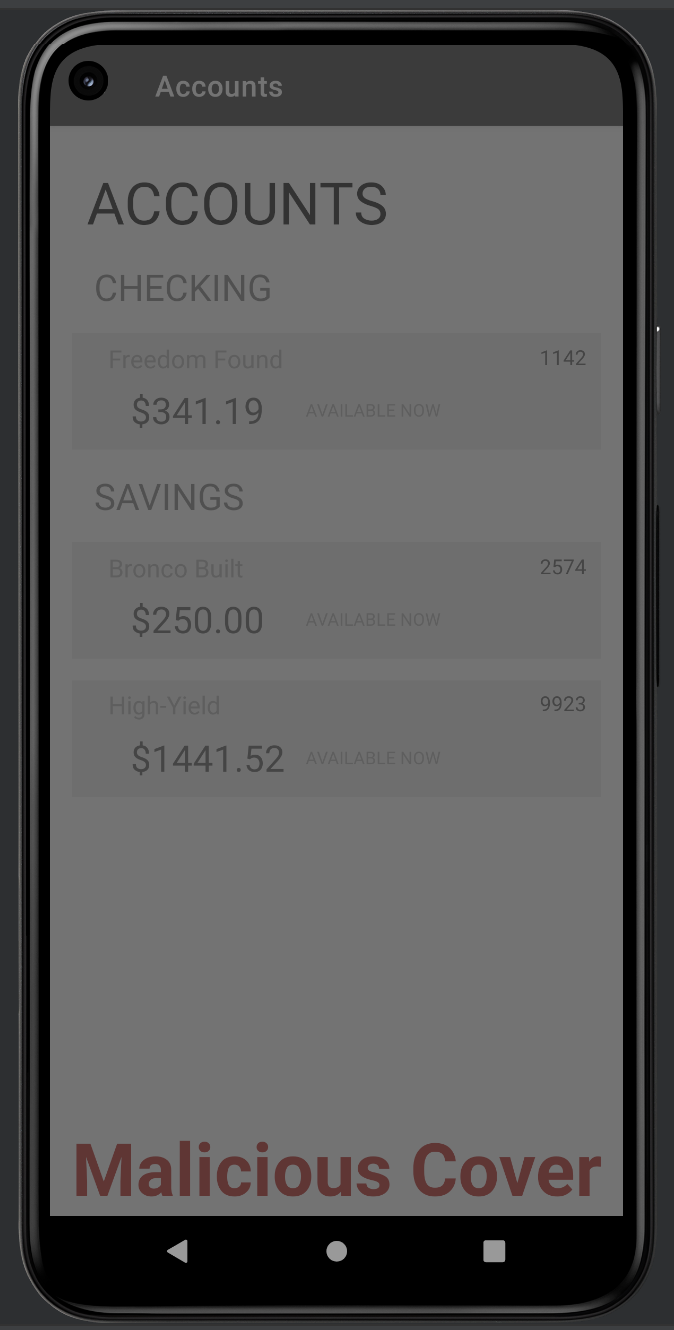
\includegraphics[scale=0.275]{graphics/malicious_cover.png}
    \caption{Example of malicious overlay}
    \label{fig:malicious_cover}
\end{figure}

\subsubsection*{Task 1.2: Input Listener: Necessary Components (Touch Modals)}\label{sec:Task-1.1-Input-Listener-Necessary-Components-Touch-Modals}
\addcontentsline{toc}{subsubsection}{Task 1.2: Input Listener: Necessary Components (Touch Modals)}

Now that your malicious app is launched over the victim application, you will now explore how to prevent the physical input listener from pausing when covered with your malicious activity. This section very similarly models the previous one; we will set flags for your malicious activity rather than the launch intent towards the victim application. Navigate to your \emph{CoveringActivity.java} file beneath the \emph{raceattack} module. The \emph{CoveringActivity.java} represents the activity that is launched over the victim application while \emph{MainActivity.java} is simply the handling application. Since this is not a launch intent, we end up setting flags for~\href{https://developer.android.com/reference/android/view/WindowManager.LayoutParams}{WindowManager.LayoutParams} (\url{https://developer.android.com/reference/android/view/WindowManager.LayoutParams}), which as the name explains, is the window manager for our activity. The functionality is very similar, minus a few minor tweaks. First and foremost, the two flags we will be setting for our window are:

\begin{itemize}
  \item \emph{WindowManager.LayoutParams.FLAG\_NOT\_TOUCH\_MODAL}
  \begin{itemize}
    \item[] This flag allows any pointer events outside of the window to be sent to the windows behind it.
  \end{itemize}
  \item \emph{WindowManager.LayoutParams.FLAG\_NOT\_TOUCHABLE}
  \begin{itemize}
    \item[] This flag leaves the touch (or ignores it) to be handled by some window below this window (in Z order).
  \end{itemize}
\end{itemize}
\bigskip

In order to set these flags to the entire activity, call the function \emph{getWindow()} and call the \emph{addFlags()} method using the dot operator behind it. The reason we call \emph{addFlags()} is because it \textit{appends} the flag codes rather than replaces them like \emph{setFlags()} does. 

\bigskip
\begin{mdframed}[backgroundcolor=blue!10,style=code,nobreak=true,align=center,userdefinedwidth=14cm]
\textbf{Action}
\bigskip

1.2.1 - Set the flags for your covering activity.
\end{mdframed}

%%%%%%%%%%%%%%%%%%%%%%%%%%%%%%%%%%%%%%%%%
%%% Task 2
%%%%%%%%%%%%%%%%%%%%%%%%%%%%%%%%%%%%%%%%%

\subsection*{Task Set 2: Creating the Overlay}\label{sec:Task Set 2: Creating the Overlay}
\addcontentsline{toc}{subsection}{Task Set 2: Creating the Overlay}

\subsubsection*{Task 2.1: Creating Instance Variable}\label{sec:Task-2.1-Creating-Instance-Variable}
\addcontentsline{toc}{subsubsection}{Task 2.1: Creating Instance Variable}

Now that we have a working overlay, we must be able to determine what to place on the screen in order to trick the user into correctly navigating to our target destination. Though the intention of the overlay is to obscure the view of the application beneath, we can determine when the application changes screens based on the triggering of the \textit{onPause()} lifecycle function.

To do so, we will create a global instance variable, wrapped in its own class, in order to keep track of each time we navigate to a different section of the application. Right click the \emph{raceattack} folder (not the module) containing all of your classes, and select 'New > Java Class'. You can name this arbitrarily. Create an instance variable \emph{screenCount} that is equal to 0, as well as an object of this class within the class's instance variables.

\bigskip
\begin{mdframed}[backgroundcolor=blue!10,style=code,nobreak=true,align=center,userdefinedwidth=14cm]
\textbf{Action}
\bigskip

2.1.1 - Create a class and a global variable to keep track of the number of screen transitions.\\
2.1.2 - Create a static public method that returns your class type called \\\emph{getInstance()}. This method should check to see if your previously created class object is null; if so, it sets instance to a new object, otherwise it simply returns the existing object.
\end{mdframed}

\begin{figure}[!ht]
    \centering
    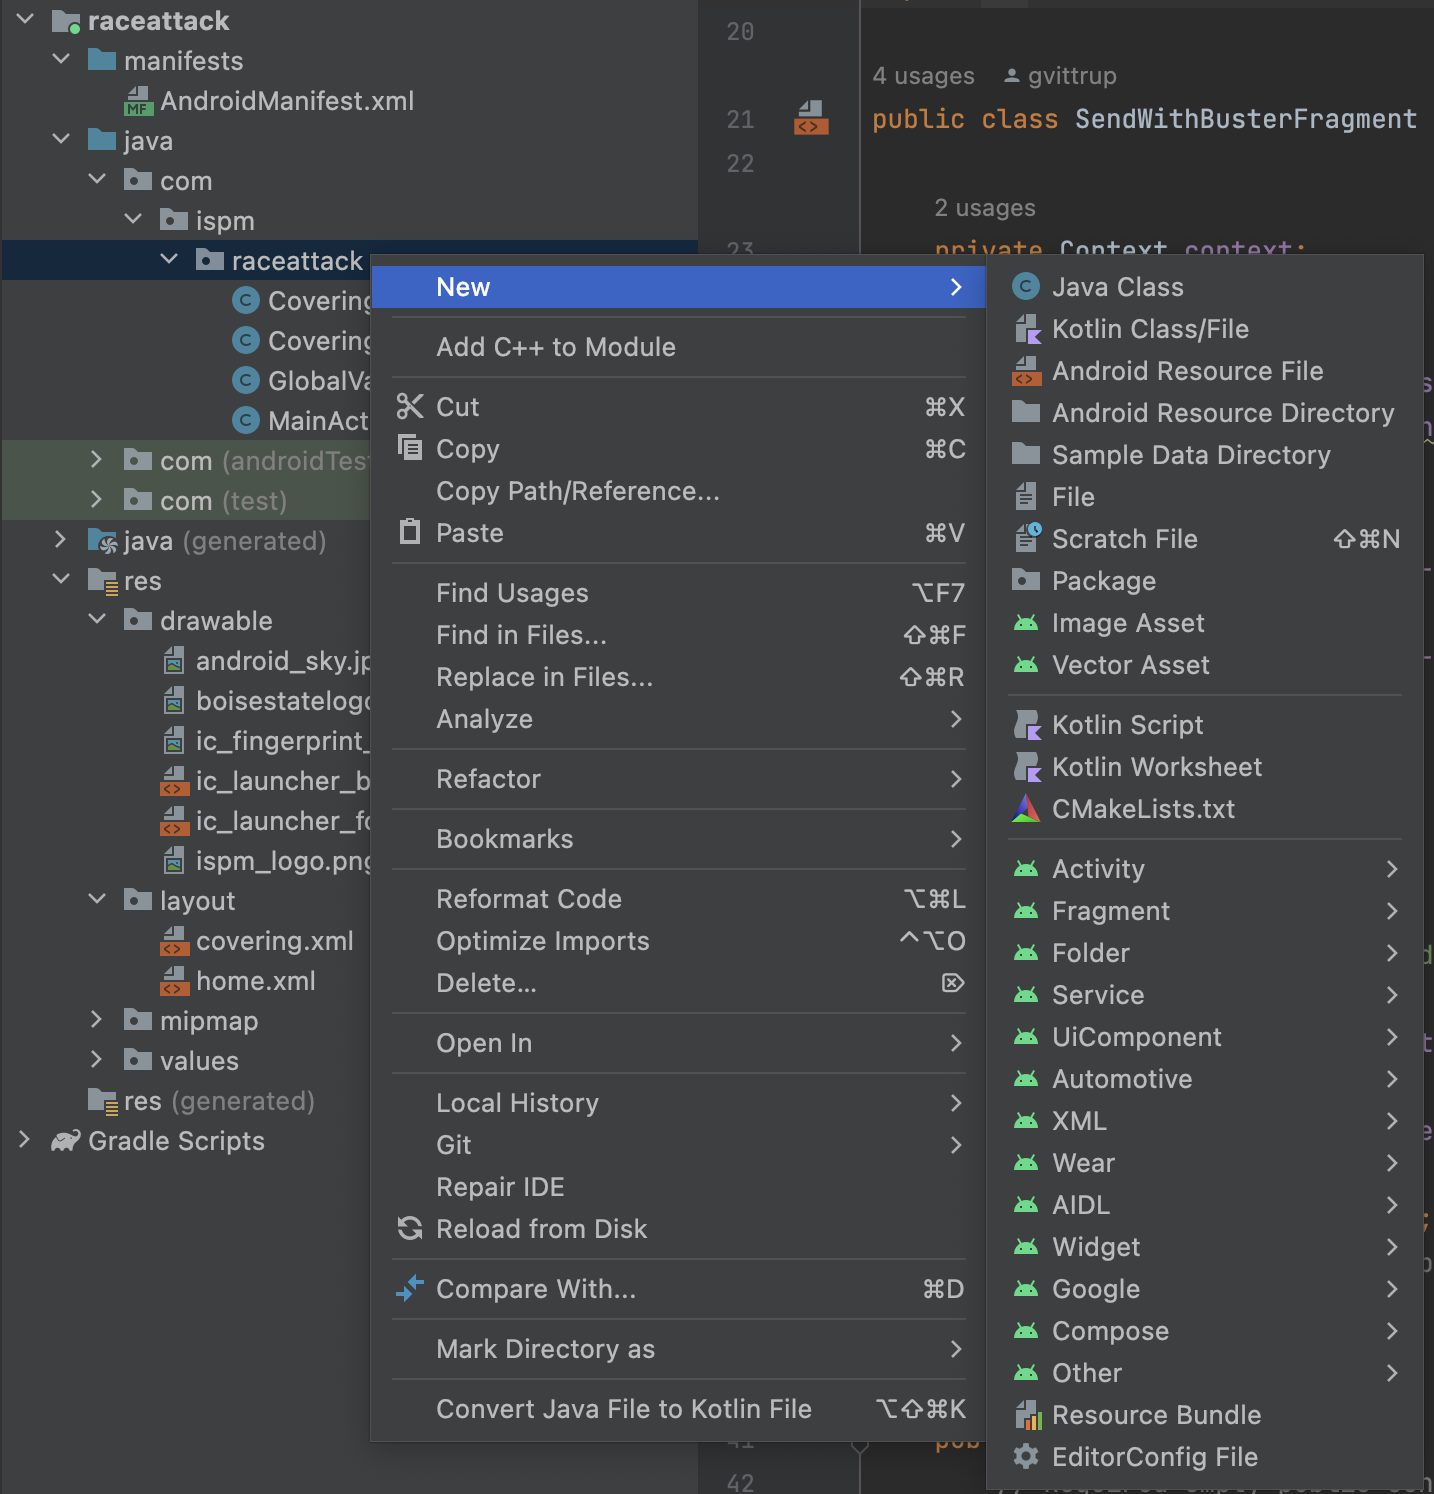
\includegraphics[scale=0.35]{graphics/java_class.png}
    \caption{Example of malicious overlay}
    \label{fig:java_class}
\end{figure}

Navigate back to your \emph{CoveringActivity.java} class. You will notice that one of your provided functions is an overridden \emph{onPause()}. This is where you will keep track of the screen count by simply calling your instanced variable \emph{screenCount}. To validate this works, follow the example code below to print to the console to ensure that it is working.

\bigskip
\begin{mdframed}[backgroundcolor=black!10,style=code,nobreak=true,align=center,userdefinedwidth=14cm]
\ Log.d("screenCount: ", GlobalVariable.getInstance().screenCount);
\end{mdframed}

\bigskip
\begin{mdframed}[backgroundcolor=blue!10,style=code,nobreak=true,align=center,userdefinedwidth=14cm]
\textbf{Action}
\bigskip

2.1.3 - Update the \textit{onPause()} function in \textit{CoveringActivity.java} to increment and log the \textit{screenCount} variable.
\end{mdframed}

\subsubsection*{Task 2.2: Creating Overlay}\label{sec:Task-2.2-Creating-Overlay}
\addcontentsline{toc}{subsubsection}{Task 2.2: Creating Overlay}

In your project window on the left-hand side, navigate to your 'res' package, and open the folder 'layout'. Beneath this, you will find your \emph{covering.xml} file. Once you open this, you will notice in the top right corner of your viewport that you have the option to change between your code and the design viewport. Here is where you will implement any respective buttons, input fields, or images to match the log-in page from the target application as much as possible. You will notice that you have a skeleton outline for a few primitive operations to get you started on utilizing these features, but any additional features or solutions can be found on the~\href{https://developer.android.com/develop/ui}{Android Studio UI documentation} (\url{https://developer.android.com/develop/ui}).

\bigskip

Now that you have a malicious application set up, it is your job to create a series of prompts that tricks the user into navigating through the application. If you explore the victim application, you will notice that it takes on the form of a student banking application. The app is kept rudimentary and only certain buttons contain functionality. The proper path to take is \emph{Transfer \& Pay -> Send with Buster -> Malicious Mallory (the greyed out option)}, and then from there you are to select an account and corresponding amount of money to take from the user. Once you click ’Send with Buster’, the application will load you to a fingerprint authorization screen, at which point you will encourage the user to enter their fingerprint. You will notice that your \emph{covering.xml} file contains some basic properties to help you get started, but it is up to you to create the entire overlay.

\bigskip

You will need to create a separate overlay for each part of the application you navigate to and change whats visible each time the screen changes. The encouraged way to implement this is by creating a section for each screen and giving it an id. Once you have done this, you will be able to toggle the visibility of each screen based on the count of your \emph{screenCount} instance variable that you created in the previous step. Create a switch case within your \emph{CoveringActivity.java} class based on \emph{screenCount} and toggle the visibility for each respective layout based on that. You can do this by mimicing the code below:

\bigskip
\begin{mdframed}[backgroundcolor=black!10,style=code,nobreak=true,align=center,userdefinedwidth=14cm]
\ findViewById(R.id.layout1).setVisibility(View.GONE);
\end{mdframed}
\bigskip

It might be preferrable to store each individual layout in a variable.

\bigskip

Because we can not determine what screen is being viewed on the application below from a zero-permission standpoint, the design is very fickle. Your overlay will only work if you successfully deceive the user into following your prompts, and otherwise will not work as intended. You are encouraged to use images, animations, timers, and any other method that will increase the effectiveness of your overlay. Create an overlay up until the final page for authorization.

\bigskip
\begin{mdframed}[backgroundcolor=blue!10,style=code,nobreak=true,align=center,userdefinedwidth=14cm]
\textbf{Action}
\bigskip

2.2.1 - Create your navigational overlay.
\end{mdframed}
\bigskip

Lastly, once you reach the authorization screen, you will notice that if you do not use the correct fingerprint or cancel the input listener, the authorization will fail. For this, the most practical way to trick a user into inputting their fingerprint is by mimicking a lock-screen. 

\bigskip
\begin{mdframed}[backgroundcolor=blue!10,style=code,nobreak=true,align=center,userdefinedwidth=14cm]
\textbf{Action}
\bigskip

2.2.2 - Create a fake lock-screen for the final destination of your overlay.
\end{mdframed}
\bigskip

%%%%%%%%%%%%%%%%%%%%%%%%%%%%%%%%%%%%%%%%%
%%% Activity Task 3
%%%%%%%%%%%%%%%%%%%%%%%%%%%%%%%%%%%%%%%%%

\break

\subsection*{Task Set 3: Game Theory}\label{sec:Task 1: Game Theory}
\addcontentsline{toc}{subsection}{Task Set 3: Game Theory}
\vspace{-0.35cm}
{\footnotesize Video: \href{https://www.youtube.com/watch?v=h3JQYd4BFGk}{\emph{Semi-Separating Equilibrium / Partially-Pooling Equilibrium by Willian Spaniel on YouTube}}}
\bigskip


Here in our last task set, we are going to explore a context and related game theory tree that will help us understand adversarial thinking between a developer and an attacker.

\begin{figure}[!ht]
    \centering
    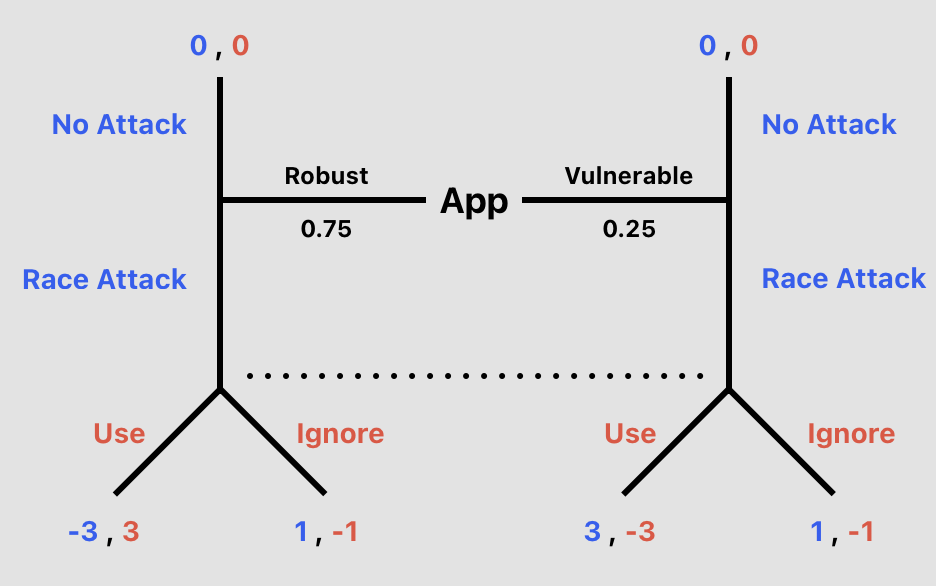
\includegraphics[scale=0.75]{graphics/PHY-game-theory-table.png}
    \caption{Game theory tree}
    \label{fig:game-theory-table}
\end{figure}

Through this game theory tree, our intention will be to find the pooling equilibrium and each players mixed strategy. The context goes as follows: An app has a 75\% chance of being robust, and a 25\% chance of being vulnerable. Player 1 (the attacker, colored in blue) decides whether or not to attack the user. The attack would be similar to our implementation, such as prompting the user to input physical touch. Player 2 (colored in red) is the user, and can decide to use (or follow) the prompt given by the attacker, or can simply ignore it. The thing is - if the user follows the attackers prompt while the app is robust, it will trigger a security flag and the attack will completely fall apart. However, if the user ignores it, the user fails to identify a malicious app on their device and provides player 1 the option of monitoring state information, thus still losing overall. If player 1 attacks a vulnerable app, regardless of player 2’s choice, player 1 will profit. Therefore, player 1 will always choose to attack.

\begin{figure}[!ht]
    \centering
    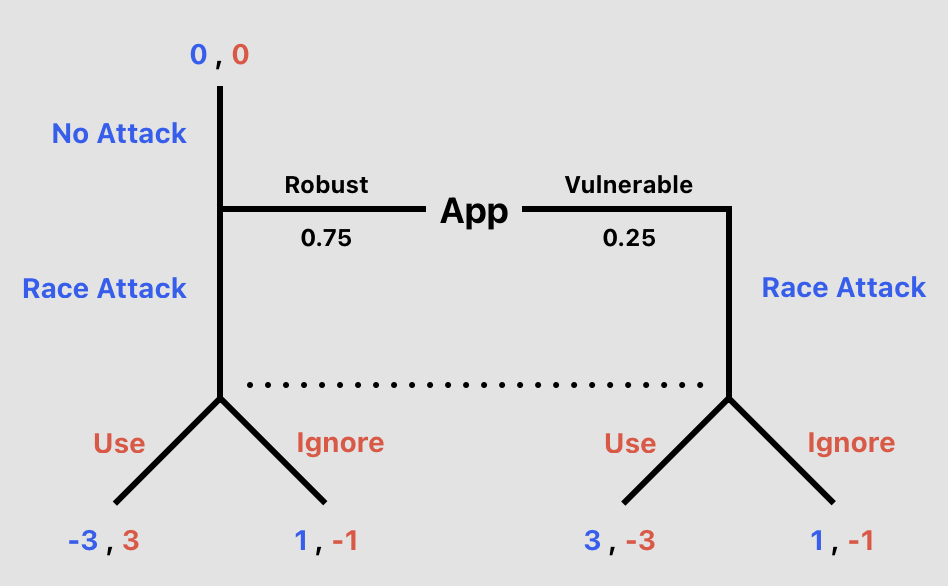
\includegraphics[scale=0.75]{graphics/PHY-game-theory-tree-v2.png}
    \caption{Player 1's profitable deviation}
    \label{fig:game-theory-tree-v2}
\end{figure}

This allows us to remove this section of the game theory tree, as we have identified that player 1 (who makes the first move) will never choose to not attack when the app is vulnerable. Now let’s consider player 2 to be an informed developer who is trying to test the security of their device and the API’s that it runs on. Let’s calculate player 2’s pooling strategy. Use the following formula below, where R signifies the probability that an app is robust, and V signifies the probability that the app is vulnerable:

$$ u(p2\_ignore) = R(p2\_ignore) + V(p2\_ignore) $$
$$ u(p2\_use) = R(p2\_use) + V(p2\_use) $$

Given player 2's pooling strategy, does player 1 have a profitable deviation? It does, because now the bluff of attacking a seemingly robust app backfires, because player 1 could stick with 0 for not attacking compared to the expected -3 if they did attack. This means we can not find any equilibria given the current information. The strategy must mix. In our game, its impossible to play a pure strategy, therefore it must mix. 
\bigskip

\begin{figure}[!ht]
    \centering
    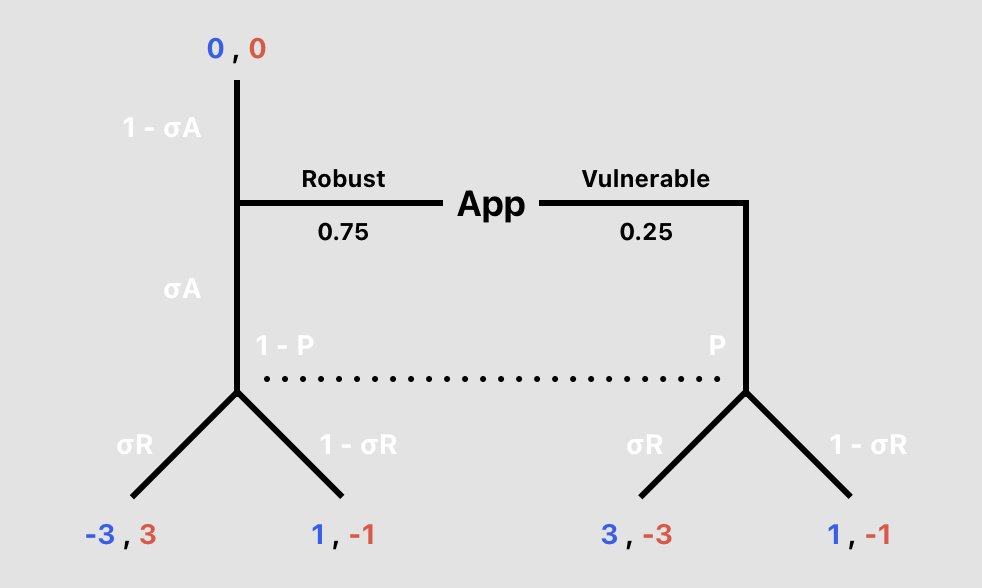
\includegraphics[scale=0.75]{graphics/PHY-tree-with-vars.png}
    \caption{Mixed strategy tree}
    \label{fig:tree-with-vars}
\end{figure}

Using this tree, we will calculate player 2's mixed strategy. To make an attack on a robust app indifferent, player 2 must mix between using and ignoring the prompt. We must calculate the utility based on player 1 attacking and their expected utility from each decision. Using indifference conditions, we can do this with the following formula:

$$ u(p1\_attack) = \sigma_R(p1\_use) + (1 - \sigma_R)(p1\_ignore) $$

We only calculate the probability for player 1's attack because if they do not attack, both players receive a utility of 0. If you work out the math, you will be left with the value of $\sigma_R$, which equals the probability that player 2 should use the app and is player 2's equilibrium strategy. But this outcome only benefits player 2 when the app is robust, therefore we need to be able to calculate player 2's belief that the app is vulnerable. Player 2's belief is represented by the variable P, and can be calculated by the following formula:

$$ u(p2\_ignore) = P(p2\_ignore) + (1 - P)(p2\_ignore) $$
$$ u(p2\_use) = P(p2\_use) + (1 - P)(p2\_use) $$

Work out the math and find the value for the variable P. This represents the portion of the time that player 2's belief is that they are facing an attack against a vulnerable app. From here, the last thing we need to do is use Bayes' rule in a non-trivial way for us to find a perfect Bayesian equilibrium. We are looking for the robust types mixed strategy that results in a value exactly equal to P found in the previous step. This can be done with the following formula:

$$ P = \frac{(0.25)(1)}{(0.25)(1) + (0.75) (\sigma_A)} $$

Add in your value for P and solve for $\sigma_A$ which represents player 1's probability that the app is robust and they attack. 

To recap:
    \begin{itemize}
        \item Player 1 attacks a robust app with a probability of $\sigma_A$
        \item After observing player 1 attack, player 2 believes that the app is vulnerable with a probability of P
        \item Player 2 then uses the app with a probability of $\sigma_R$
    \end{itemize}

\bigskip
\bigskip
\bigskip

\begin{mdframed}[backgroundcolor=blue!10,style=code,nobreak=true,align=center,userdefinedwidth=14cm]

\textbf{Action}
\bigskip

3.1.1 - Calculate player 2's pooling equilibrium.\\
3.1.2 - Which strategy profitably deviates?\\
3.1.3 - Calculate the value of $\sigma_R$, which represents player 2's mixed equilibrium strategy.\\
3.1.4 - What is the probability that player 2 uses the app?\\
3.1.5 - Calculate the value of P, which represents player 2's belief that they are facing a vulnerable app.\\
3.1.6 - Calculate the value of $\sigma_A$, which represents the probability that the app is robust and player 1 chooses to attack.
\end{mdframed}

\subsection*{Summary}\label{sec:Summary-MS}
\addcontentsline{toc}{subsection}{Summary}

Many mobile apps use these physical interfaces to receive user-input for authentication/authorization operations including one-click login, fingerprint-based payment approval, and face/voice unlocking. Our focus on this activity was to mislead an unsuspecting user with a zero-permission malicious application to feed screen-touch and fingerprint input in order to unintentionally authorize a fund-transfer. Furthermore, we explored some conventional design patterns that led to increased security risks regarding these types of attacks.

\subsection*{Trouble Shooting}\label{sec:Trouble Shooting}
\addcontentsline{toc}{subsection}{Trouble Shooting}
    
\subsubsection*{Refactoring the Project Name}
\addcontentsline{toc}{subsubsection}{Refactoring the Project Name}

Make sure you change the respective lines within build.gradle and AndroidManifest.xml to match what you refactored your project to. Then, select File->Invalidate Caches->Restart, and your project should rebuild with the correct dependencies. If this does not work, you can select Build->Clean Project and Build->Rebuild Project and then retry invalidating the caches. This will fully correct your problem.

\subsubsection*{Images: 'Trying to render too large of a bitmap' error}
\addcontentsline{toc}{subsubsection}{Images: 'Trying to render too large of a bitmap' error}

Scroll down to your ‘res’ folder, right click, and create new Android Resource Folder. Select the dropdown and click ‘Drawable’. In the navigator pane on the bottom left, scroll down and select ‘Density’. This will create a ‘Drawable-xxxhdpi’ folder. Now, navigate to your drawable in the ‘Resource Manager’, right click, and move the file into that newly created folder. If this does not work, delete your image, reupload it, and before importing it change its version to ‘UI Mode’. Repeat the previous process and everything should work as intended.

\bibliography{References}
\bibliographystyle{plain}

\end{document}

%%%%%%%%%%%%%%%%%%%%%%%%%%%%%%%%%%%%%%%%%